\chapter{Methodology}
\label{ch:Methodology}
This chapter outlines the methodologies used throughout the project to achieve the research objectives and answer the thesis questions concerning image quality assessment (IQA) in teledermatology. It discusses the exploratory approach adapted during the project, characterized by cycles of decision-making and agile methodologies.\par

\section{Explorative Approach}
\label{sec:ExplorativeApproach}
Teledermatology, particularly focused on IQA, presents a broad scope for innovation due to the variety of possible image distortions and the different ways these can be addressed. The exploratory approach adopted in this research is characterized by its high degree of innovation and flexibility, which sometimes comes at the expense of linearity. Traditional phased approaches are not always applicable, leading to the adoption of a methodology based on explorative cycles with decision-making processes and agile practices. \par
\vspace{\baselineskip}
\noindent
Initially, the problem statement for this project was only broadly defined, setting the stage for an adaptive and fluid approach as the research unfolded. As the project progressed, it increasingly focused on creative problem-solving, facilitated through multiple learning cycles that allowed for iterative refinement of ideas and methods. The research was structured into two distinct phases to manage this process effectively. In the early stages, known as the Diverging Phase, the scope of the research question was deliberately expanded. This expansion enabled the continuous generation of new ideas, each informed by the insights gathered during the ongoing investigation. Later, in the Converging Phase of the project, the emphasis shifted towards synthesizing these ideas into a cohesive set of findings and conclusions, aiming to consolidate the diverse insights into a unified understanding of the initial problem statement (\cite{DesignThinking}). A schematic of this exploratory model is depicted in  \autoref{fig:decision_cycle}.\par
\begin{figure}[ht]
    \centering
    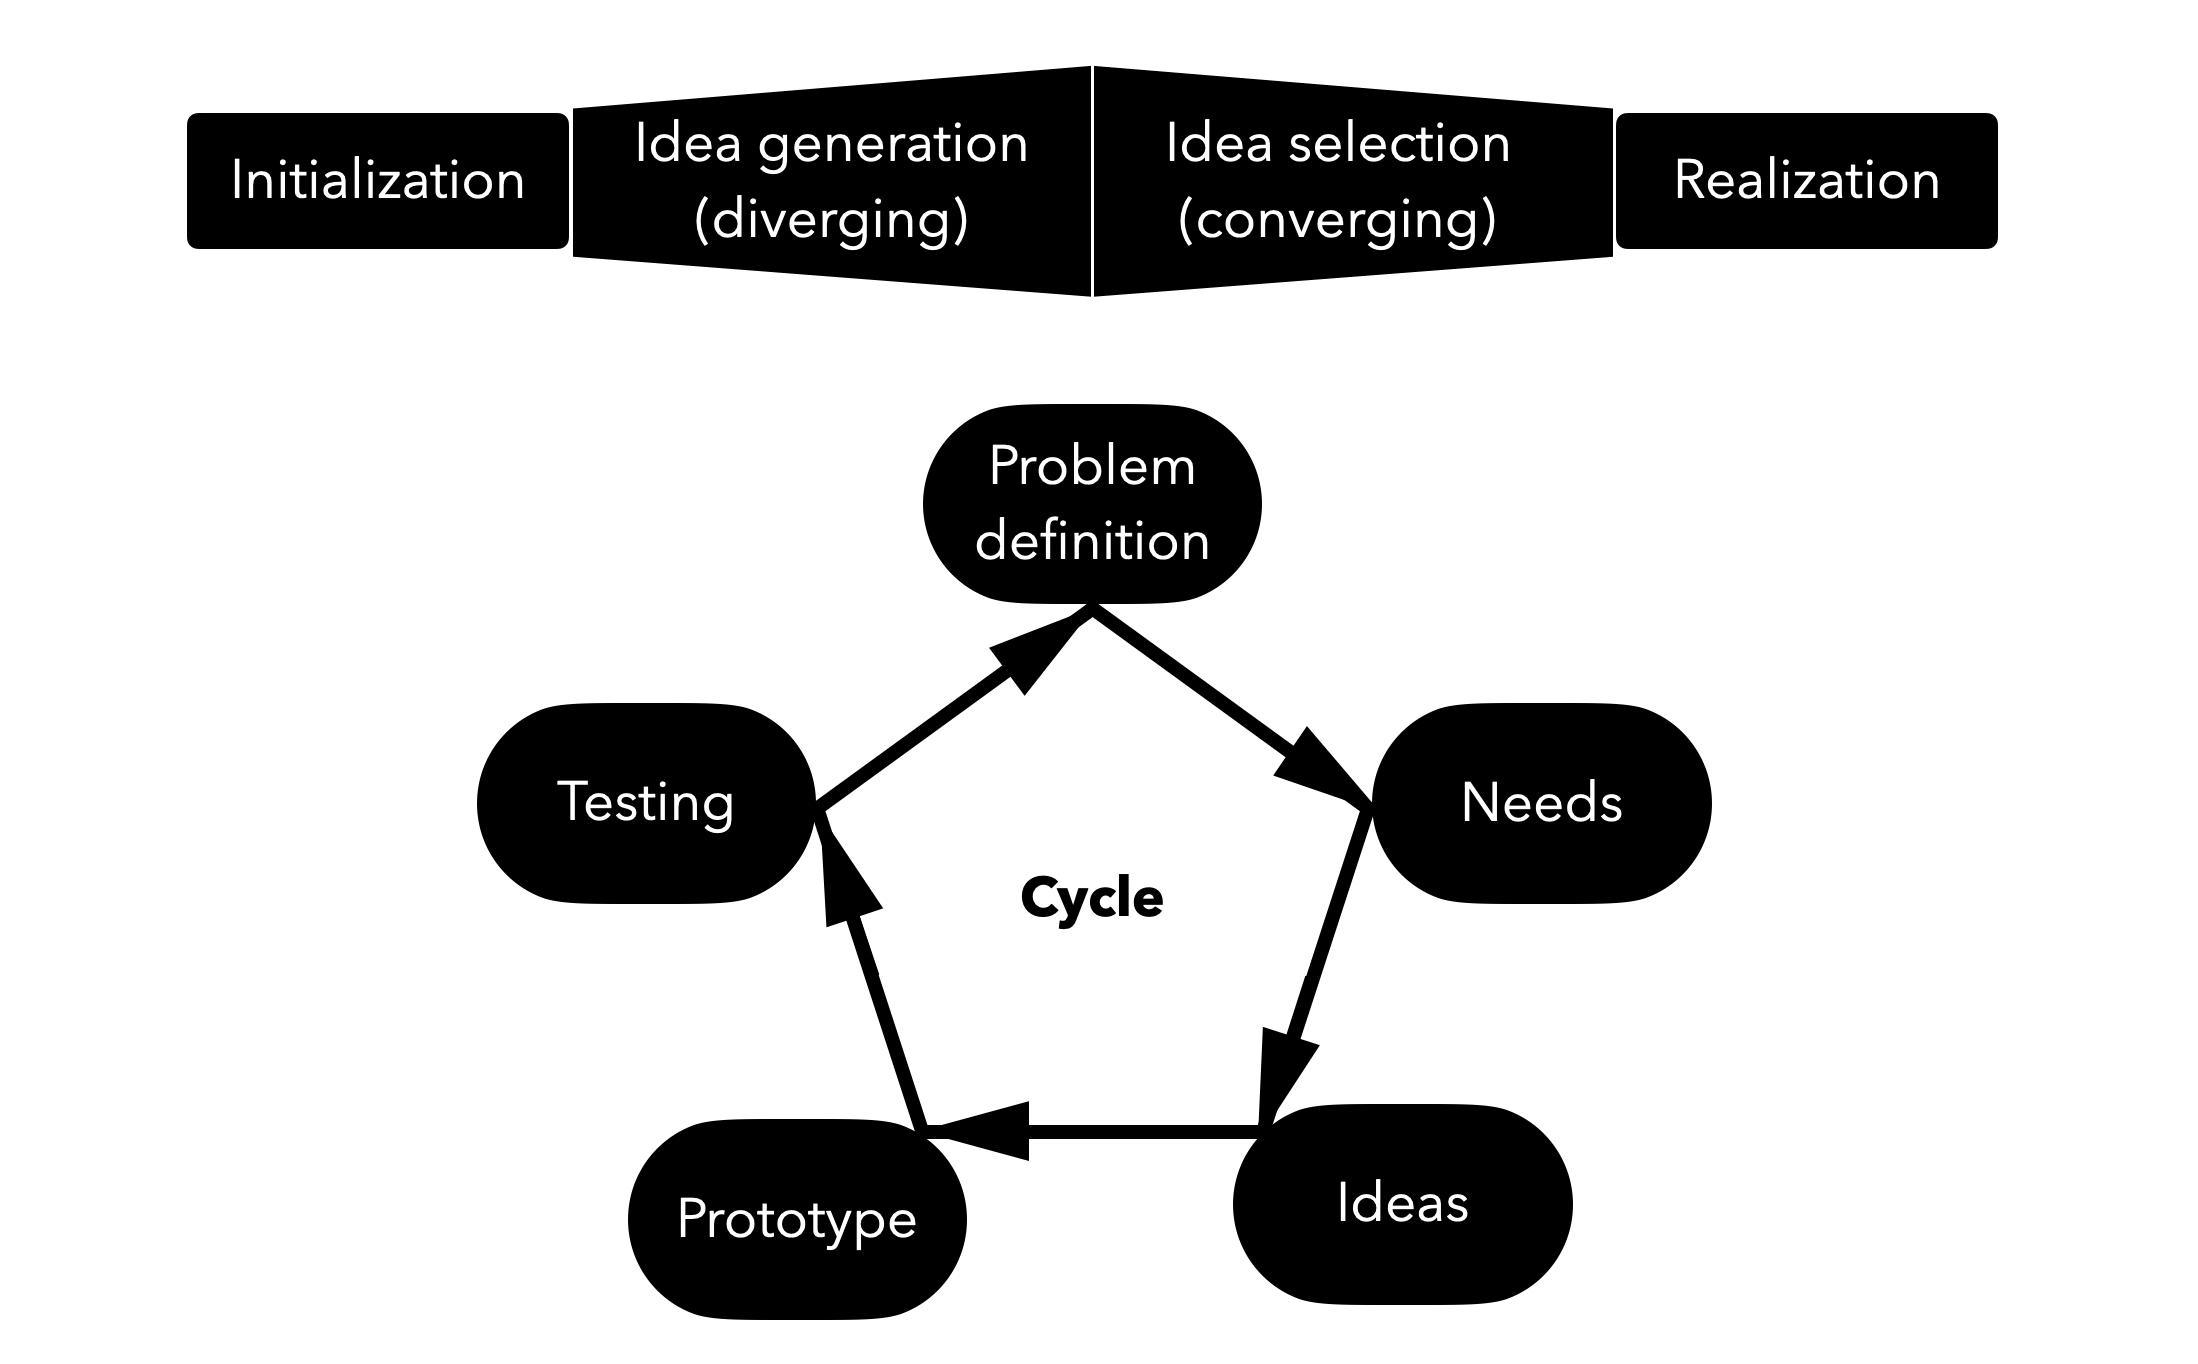
\includegraphics[keepaspectratio,width=15cm]{img/DecisionCycle.png}
    \caption{Illustration of the explorative approach, including the stages of initialization, idea generation, idea selection, and implementation. The lower part of the figure shows the decision cycles (\cite{DesignThinking}).}
    \label{fig:decision_cycle}
\end{figure}

\section{Project Control}
\label{sec:ProjectMonitoring}
Despite the exploratory approach's lack of traditional milestones, it is crucial to have a rough timeline to successfully navigate the research tasks. Before commencing, a workflow was established, detailed in the planning document attached to this thesis. There are three essential milestones identified in the first half of the project, each critical to its success: \par
\vspace{\baselineskip}
\noindent
\textbf{Understanding Teledermatology}: Gaining a deep understanding of the domain to ensure all subsequent actions are relevant and informed. \par
\noindent
\textbf{State of the Art in IQA}: Identifying the latest developments in IQA to ensure the methods used are cutting-edge. \par
\noindent
\textbf{Availability of Teledermatology Data}:  Ensuring access to appropriate datasets for conducting meaningful IQA. \par
\vspace{\baselineskip}
\noindent
These milestones are pivotal as each subsequent phase relies on the successful completion of the previous. Failure to achieve these could severely impact the project, potentially necessitating a fundamental reassessment of the objectives according to (\autoref{sec:Objectives}). \par

\section{Research Steps}
\label{sec:ResearchSteps}
Due to the explorative nature of this study, a linear progression through predefined research steps was not feasible. However, key steps were categorized and executed as follows:

\subsection{Literature Review}
\label{sub:LR}
The literature review is foundational to the research, setting the stage for framing the research questions and determining the appropriate methodologies. This initial phase involved a thorough examination of existing research on IQA, focusing specifically on methodologies previously employed and their effectiveness within teledermatology. By analyzing these methodologies, the review highlighted both their strengths and limitations, providing a nuanced understanding of the current landscape and the gaps in knowledge and application.\par
\vspace{\baselineskip}
\noindent
The choice of ARNIQA as the primary methodological tool for this thesis was influenced significantly by the insights gained from the literature. ARNIQA's advanced capabilities in handling a range of image distortions—which are critical for teledermatology—made it an ideal choice. Traditional IQA methods often fall short in managing the complex and varied image qualities encountered in teledermatology; however, ARNIQA, with its robust image degradation model and its use of SimCLR for learning from unlabeled images through contrastive learning, offers a substantial improvement. This approach is particularly advantageous in scenarios where high-quality labeled datasets are scarce or incomplete. \par
\vspace{\baselineskip}
\noindent
The literature review not only reinforced the methodology’s alignment with the project's aims but also highlighted ARNIQA’s potential to enhance current IQA practices in teledermatology. This phase was crucial for ensuring that the subsequent steps were built on a solid theoretical foundation, guided by informed insights into the state of the art, and tailored to meet the specific demands of assessing image quality in a teledermatological context. The outcomes of this foundational step provided the necessary groundwork for the detailed investigations and methodological applications that followed. \par
\vspace{\baselineskip}
\noindent

\subsection{Data Collection and Preparation}
\label{sub:DataCollection}
In the pursuit of a suitable dataset for evaluating image quality within teledermatology, a significant challenge encountered was the absence of teledermatology datasets that included Mean Opinion Score (MOS) or Differential Mean Opinion Score (DMOS) similar to those commonly available in traditional IQA datasets (\autoref{sub:BenchmarkDatasetsIQA}). This scarcity is largely due to the clinical nature of most teledermatology images, which are often captured using dermoscopes in controlled settings, thereby not representing the typical use case in remote dermatological assessments.\par
\vspace{\baselineskip}
\noindent
To address this gap, the SCIN dataset was chosen for its relevance and uniqueness. Unlike many dermatological datasets that predominantly focus on skin cancer diagnostics through the classification of malignant and benign tumors, the SCIN dataset encompasses a broader spectrum of common dermatological conditions. These conditions primarily include allergic, inflammatory, and infectious diseases, which are frequently encountered in everyday clinical practice but underrepresented in existing datasets. What makes the SCIN dataset particularly valuable for this research is that it captures images of early-stage concerns—over half of the images were taken less than a week from the onset of symptoms, with 30\% captured less than a day after. These are conditions patients are likely to consult via teledermatology platforms before they could be seen in a traditional healthcare setting.\par
\vspace{\baselineskip}
\noindent
Given the project's focus on image quality assessment rather than diagnostic accuracy, I adapted the SCIN dataset for my specific research needs. This adaptation involved creating two distinct sets of images:\par
\vspace{\baselineskip}
\noindent
\textbf{Good Quality Set}: This set was compiled based on my assessment of what constitutes 'good quality' in dermatological images. Although I am not a dermatologist, the selection was guided by general quality criteria relevant to both clinical and non-clinical settings. \par
\noindent
\textbf{Test Set with Labeled Images}: To quantitatively assess image quality, I personally labeled a test set, applying scores from 0 to 1 for each of the seven quality criteria (\autoref{sub:QualityCriteriaTeledermatology}) identified as critical for teledermatology. In this scoring system, a score of 1 indicates extreme distortion relevant to the specific criterion, and a score of 0 signifies no noticeable distortion.
\par
\vspace{\baselineskip}
\noindent
This approach to dataset preparation not only tailored the data to the specific needs of this research but also established a framework for systematically assessing image quality in teledermatology. This preparation is crucial for the next phases of the project, which involve training and validating the image quality assessment model to ensure it can reliably perform in real-world teledermatology applications. \par


\subsection{Training and Validation}
\label{sub:TrainVal}
The model training process begins with the application of a series of predefined distortions to a set of high-quality images. These distortions are carefully selected to simulate real-world imperfections commonly encountered in teledermatology. Each image is then labeled according to the severity and type of distortion applied, creating a dataset that not only includes the distorted images but also features precise annotations regarding their quality.
\par
\vspace{\baselineskip}
\noindent
Feature extraction is a critical next step where the SimCLR model from ARNIQA is utilized to derive meaningful representations from the distorted images. These features are expected to capture the underlying patterns of distortions that affect image quality. \par

\subsubsection{Overview of Training and Validation Processes}
\label{subsub:OverciewTrainVal}
\textbf{Model Selection and Training}: A regression model will be employed to correlate the extracted features with the labeled image quality scores. The choice of model—be it a Random Forest or a Linear Regressor—will be based on a balance of accuracy, interpretability, and computational efficiency. This model will learn to predict the quality of an image, effectively turning the features extracted by SimCLR into actionable insights. \par 
\noindent
\textbf{Validation Strategy}: Validation plays a crucial role in ensuring that the model not only performs well on the training data but is also effective and reliable when deployed in real-world teledermatology settings. The model will be validated using a separate set of images that were not included in the training phase. Standard statistical metrics such as accuracy, precision, and recall, among others, will be used to evaluate the model’s performance, ensuring its efficacy and robustness.\par
\vspace{\baselineskip}
\noindent
For a comprehensive understanding of the specific methodologies employed — including the intricacies of the distortion pipeline, the operational details of SimCLR, and the exact validation protocols — please refer to the Implementation section (\autoref{ch:Implementation}). This section will delve into the technical specifics, providing a detailed description of each step involved in the process, from the initial data handling to the final stages of model evaluation. \par 


\subsection{Testing and Experiments}
\label{sub:TestExperiment}
The testing and experimental phase of the research is crucial for validating the efficacy and accuracy of the image quality assessment model developed in the previous stages. The testing phase employs a set of images that I personally labeled based on seven critical quality criteria for teledermatology, with scores ranging from 0 (no distortion) to 1 (extreme distortion). This phase evaluates the model’s ability to assess image quality accurately, using metrics such as Mean Squared Error (MSE) and R-Squared. These metrics will help determine how well the model's predictions align with the actual labels, providing a baseline for assessing the model’s performance and guiding future improvements. Detailed procedures and metrics will be elaborated further in the Implementation section (see Section \autoref{ch:Implementation}).\par 

\subsection{Discussion and Further Development}
\label{sub:DiscussionDevelopment}
The final phase of the project involves analyzing and discussing the results obtained from the model testing. This discussion will assess how effectively the model meets the research objectives and will highlight areas where the model excelled or fell short. Insights gained from this analysis will inform potential areas for further development, such as refining the model's ability to handle specific distortions or improving its generalization across diverse teledermatology images. This ongoing cycle of evaluation and enhancement is crucial for advancing the field of image quality assessment in teledermatology, ensuring that the methodologies continue to evolve in line with technological advancements and clinical needs. \par




\vspace{\baselineskip}
\noindent
\textbf{Note:} \par
\vspace{\baselineskip}
\noindent
The approach to training and validation in this thesis involves a novel method of applying and assessing distortions based on the defined quality criteria critical to teledermatology. The process begins by taking good quality images and subjecting them to a systematic distortion pipeline, which is designed to simulate real-world imperfections that could affect diagnostic accuracy in teledermatology.\par
\noindent
Distortion Implementation:\par
Each of the seven quality criteria identified has a corresponding distortion type, such as motion blur for focus. These distortions are quantified across five levels, from 0 (no distortion) to 8 (severe distortion). The application of these distortions is controlled by a probabilistic model based on a Gaussian distribution, with a mean of 0 and a standard deviation of 2.5. This statistical approach ensures a natural variability in the application of distortions, closely mimicking the random nature of image quality issues in practical settings.\par
\noindent
The specific levels of distortion for each image are selected using normalized probabilities, ensuring that each level of severity has a realistic chance of being applied. The distortions are then applied to the images, and each image is labeled with values scaled between 0 to 1 corresponding to the severity of the applied distortions, with these labels indicating the level of quality degradation for each criterion.\par
\noindent
Feature Extraction and Regression Model Training:\par
Once the images have undergone distortion, they are processed through the SimCLR framework from ARNIQA to extract features. SimCLR is particularly suited for this task as it is designed to learn useful representations from unlabeled data in an unsupervised manner, making it ideal for scenarios where explicit labels might not be available or fully reliable.\par
\noindent
The extracted features, along with the generated labels, are then used to train a regression model. The choice of the regression model, whether it be a Random Forest or a simple Linear Regressor, will depend on the performance criteria such as accuracy and computational efficiency. The regression model will learn to predict the quality level of an image based on the features extracted by SimCLR, which are indicative of the various distortions applied.\par
\noindent
Validation:\par
The validation phase involves assessing the trained model's accuracy and its ability to generalize across different sets of images. This is crucial for ensuring that the model performs well not only on the training data but also on unseen images, which would be representative of a real-world application in teledermatology. The model's performance is evaluated using standard metrics such as Mean Squared Error (MSE) or R-squared, which provide insights into how well the model predicts image quality.\par
\noindent
This training and validation process is critical as it directly influences the reliability and effectiveness of the IQA in a teledermatology context. It ensures that the system can accurately identify and quantify the severity of various distortions, thus supporting dermatologists in making informed decisions based on the quality of the images they review.\par
\noindent
Considerations:\par
It's essential to ensure that the distribution and application of distortions during the training phase closely mimic realistic scenarios to prevent the model from overfitting to unrealistic patterns. Additionally, considering ethical aspects and the potential impact on patient outcomes, it is crucial to maintain high accuracy and reliability in the model's predictions to support effective and safe teledermatology practices.\par
Literature Review on IQA and Teledermatology \par
Purpose: Start by discussing the significance of the literature review in framing your research questions and methodology.\par
\noindent
Content: Outline how the literature influenced the selection of your methods and tools, particularly focusing on past approaches to IQA and their applicability or limitations in teledermatology.\par
\noindent
Rationale: Explain the choice of ARNIQA based on gaps or strengths identified in the literature, establishing why it's well-suited for addressing current challenges in teledermatology image quality assessment.\par
\noindent
Image Quality Assessment Methodology \par
Introduction to ARNIQA: Detail why ARNIQA was chosen for IQA in teledermatology, emphasizing its strengths such as the sophisticated image degradation model and its ability to train with fewer labeled examples.\par
\noindent
Explaining SimCLR: Provide an in-depth explanation of SimCLR, discussing how it works (contrastive learning mechanism), why it is effective (ability to learn useful representations from unlabeled data), and its particular advantages for your research (e.g., robustness to various distortions).\par
\noindent
Utility and Implementation: Describe how you implemented ARNIQA and SimCLR, including any modifications or optimizations made for teledermatology. Mention the availability of code and weights, which ensures reproducibility and facilitates future research.\par
\noindent
Teledermatology Image Quality Assessment \par
Dataset Description: Introduce the SCIN dataset, explaining why it's suitable for your study, its composition, and any preprocessing steps involved.\par
\noindent
Distortion Model Creation: Discuss the design of your custom distortion model, detailing the types and layers of distortions you included. Justify why these particular distortions are relevant to teledermatology.\par
\noindent
Test Set and Labeling: Explain how you created and labeled your test set, including the criteria used for labeling and the process of validation.\par
\noindent
Architecture Overview: Provide a comprehensive overview of the entire system architecture, showing how each component (data input, processing, analysis, and output) integrates to form a cohesive workflow. \par
\noindent
Summary of Methodological Approach \par
Synthesis: Briefly summarize how each part of your methodology contributes to addressing the research questions or hypotheses stated in earlier chapters.\par
\noindent
Justification: Reinforce the rationale behind your methodological choices, linking back to the literature review and the specific challenges identified in teledermatology IQA.\par